\documentclass[./MATH-115-Notes.tex]{subfiles}
\begin{document}
\chapter{Chapter 10: Parametric Equation and Polar Coordinates}
So far we have described curves by giving $y$ as a function of x, i.e. $y = f(x)$ or $x$ as a function of y, i.e. $x = g(y)$, or by giving a relation between x and y that defines y implicitly as a function of x like $y^2 + x^2 = 1$.
\\~\\ 
Some curves, such as the cycloid, are best handled when both  and  are given in terms of a third variable $t$ called a parameter, i.e. $x = f(t),\ y = g(t)$.
\section{Parametric Curve}
\begin{paperbox}{Notation}
    \begin{equation}
        C = (x(t), y(t))
    \end{equation}
    $ x = x(t) $ ,$ y = y(t) $ are functions of parametric t
\end{paperbox}

\subsection{Position and speed of a particle in orbit}
Lets say that the x position of the particle can be defined as $x = \cos(2t)$ and the y position can be defined as $ y = \sin(2t) $. Then we have a parameter curve that is defined as $C = (\cos(2t), \sin(2t)) $. \\
This is what the parameter curve would look like from $ 0 \leq t \leq 2\pi$:\\
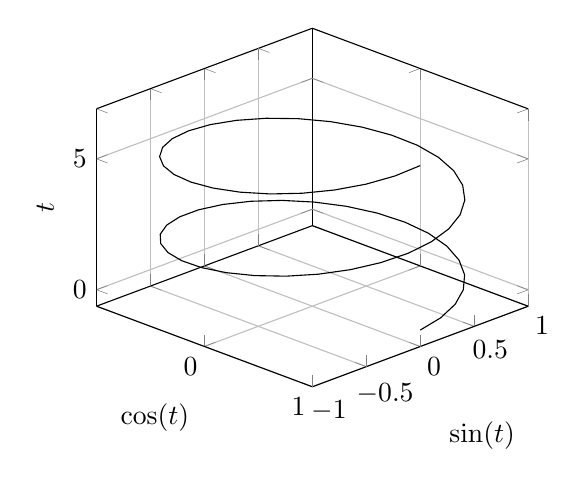
\begin{tikzpicture}
    \begin{axis}
        [
        scale=0.8,
        grid,
        view={45}{30},
        xlabel=$\cos(t)$,
        ylabel=$\sin(t)$,
        zlabel=$t$,
        ]
    \addplot3[
        domain=0:2*pi,
        samples = 60,
        samples y=0,
    ]
    ({cos(deg(2*x))},
    {sin(deg(2*x))},
    {x});
    \end{axis}
\end{tikzpicture}
\newpage
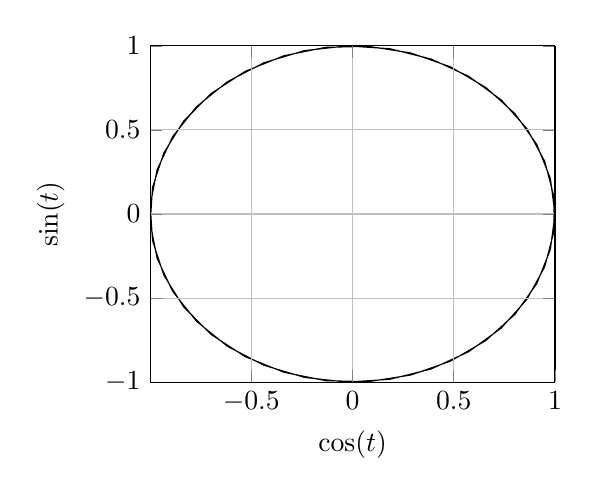
\begin{tikzpicture}
    \begin{axis}
        [
        scale=0.75,
        grid,
        view={0}{90},
        xlabel=$\cos(t)$,
        ylabel=$\sin(t)$,
        ]
    \addplot3[
        domain=0:2*pi,
        samples = 60,
        samples y=0,
    ]
    ({cos(deg(2*x))},
    {sin(deg(2*x))},
    {x});
    \end{axis}
\end{tikzpicture}
It creates a circle.

\subsubsection{Velocity Vector and Speed}
\begin{paperbox}{The Velocity Vector Equation}
    The velocity of the particle can be figured out by finding the rate of change on both the x and y axes. This will give us a vector that is the tangential velocity of the particle at a given time t.
    \begin{equation}
        \vec{V} = < x'(t), y'(t) >
    \end{equation}
    To get the speed we take the magnitude of the velocity vector
    \begin{equation}
        V = || \vec{V} || = \sqrt{ (x'(t))^2 + (y(t))^2 }
    \end{equation} 
\end{paperbox}
For the previous example, the equation for the velocity vector and speed is:
\begin{gather*}
    \vec{V}(t) = <(\cos(2t))', (\sin(2t))'>\\
    \vec{V}(t) = <-2\sin(2t), 2\cos(2t)>\\
    V(t) = \sqrt{(-2\sin(2t))^2 + (2\cos(2t))^2}\\
    V(t) = \sqrt{4\sin^2(2t) + 4\cos^2(2t))}\\
    V(t) = \sqrt{4\ (\sin^2(2t) + \cos^2(2t)))}\\
    V(t) = \sqrt{4}\\ 
    V(t) = 2
\end{gather*} 
\newpage   
\subsection{Tangent line}
\begin{paperbox}{Tangent line equation}
    \begin{equation}
        m = \frac{dy}{dx} = \frac{dy\cancel{/dt}}{dx\cancel{/dt}}
    \end{equation}
    Tangent line equation
    \begin{equation}
        y - y_0 = m(x - x_0)
    \end{equation}
\end{paperbox}
\subsubsection{Example}
Find the tangent of this parametric equation $ C = (2\cos(3t), 2\sin(3t)) $ when $t = \frac{\pi}{3}$ and $t = \frac{\pi}{6}$
\\~\\
First we need to find $P_0$ and $P_1$ for the two times.
$$
    P_1 = 2\cos\biggl(3\frac{\pi}{3}\biggl), 2\sin\biggl(3\frac{\pi}{3}\biggl) \rightarrow P_0 = (-2,0)
$$

$$
    P_2 = 2\cos\biggl(3\frac{\pi}{6}\biggl), 2\sin\biggl(3\frac{\pi}{6}\biggl) \rightarrow P_1 = (0,2)
$$

Now we need to find the slope.

$$
    m = \frac{\cancel{6}\cos(3t)}{\cancel{6}-\sin(3t)} \Rightarrow m = -\frac{cos(3t)}{\sin(3t)}
$$
\begin{gather*}
    m_1 = -\frac{cos(3(\pi/3))}{\sin(3(\pi/3))} = \frac{1}{0} = \infty\\
    m_2 = -\frac{cos(3(\pi/6))}{\sin(3(\pi/6))} = -\frac{0}{1} = 0
\end{gather*}
Inputting the slopes into our tangent line equation gives us
\begin{gather*}
    y_1 = \infty(x+2) \Rightarrow \frac{y_1}{\infty} = x + 2\\
    0 = x + 2 \Rightarrow x = -2\\
    y_2 = 0(x-2)
\end{gather*}
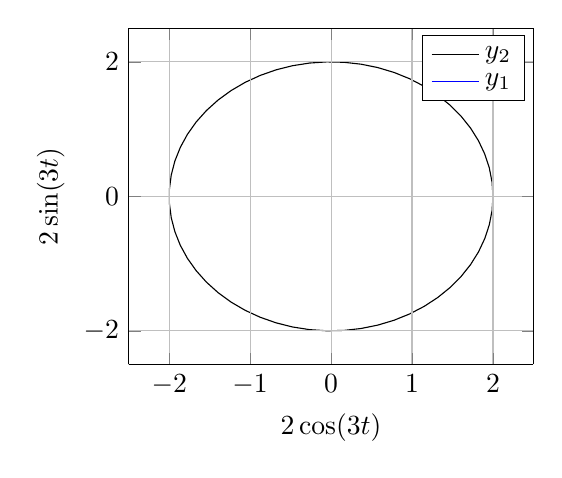
\begin{tikzpicture}
    \begin{axis}
        [
        scale=0.75,
        grid,
        view={0}{90},
        xmin=-2.5,ymin=-2.5,xmax=2.5,ymax=2.5,
        xlabel=$2 \cos(3t)$,
        ylabel=$2 \sin(3t)$,
        ]
    \addplot3[
        domain=0:2*pi,
        samples = 60,
        samples y=0,
    ]
    ({2 *cos(deg(x))},
    {2 * sin(deg(x))},
    {x});
    \addplot[blue]
    {2};
    \addlegendentry{$ y_2$}
    \addplot3[red]
    ({-2},{x},{x});
    \addlegendentry{$ y_1 $}
    \end{axis}
\end{tikzpicture}
\newpage




\subsection{Concavity}
To find the concavity of a parametric curve you find the second-order derivative of the curve. This is different than finding the second-order derivative of a regular function.   
\begin{paperbox}{Second-order derivative of a parametric curve}
    Because you are trying to find the second-order derivative with respect to x, you have to arrange the expression as such.
    \begin{gather*}
        \frac{d^2y}{dx^2} = \frac{d}{dt}\biggl(\frac{dy(t)}{dx(t)}\biggl)\frac{dt}{dx}\\
        = \frac{\frac{dy'(t)}{dtx'(t)}}{\frac{dx}{dt}}\\
        \text{Using the quotient rule gives you}\\
        = \frac{\frac{y''(t)x'(t) - y'(t)x''(t)}{(x'(t))^2}}{x'(t)}
    \end{gather*}
    \begin{equation}
        \frac{d^2y}{dx^2} = \frac{y''(t)x'(t) - y'(t)x''(t)}{(x'(t))^3}
    \end{equation}
\end{paperbox}

\subsubsection{Example}
For this parametric curve $ C = (t^2, t^3 - 3t) $.
\begin{enumerate}[label=\alph*)]
    \item Find for all t such that the curve passes though (3,0)
    \item Find the tangent line that all pass though (3.0)
    \item Find points where the tangent line is horizontal and vertical
    \item Find the intervals where it concave up and down
\end{enumerate}
\textbf{Solution}\\
\noindent
a) This is simple, find t such that it will satisfy the point.
$$
    3 = t^2 = \pm \sqrt{3}
$$
b) Using the slope equation from the last subsection gives us this expression:
$$
    \frac{3t^2-3}{2t} = m(t)
$$
Input both values of $t$ into the slope equation gives us these values for the slope:
\begin{gather*}
    \frac{3(-\sqrt{3})^2-3}{2\cdot-\sqrt{3}} = -\sqrt{3}\\
    \frac{3(\sqrt{3})^2-3}{2\sqrt{3}} = \sqrt{3}
\end{gather*}
Therefore, the tangent lines are 
\begin{gather*}
    y_1 = \sqrt{3}(x - 3)\\
    y_2 = -\sqrt{3}(x - 3)
\end{gather*}
c) Set the slope $m = 0$, then you have:
\begin{gather*}
    0 = \frac{3t^2-3}{2t}\\
    t = \pm 1 \\
    \text{Input t into the orginal equation}\\
    P_{horizontal} = ( (\pm 1)^2 , (\pm 1)^3 - 3(\pm 1) )\\
    P_{horizontal} = 
    \begin{cases}
    (1, -2)\\
    (1, 2)    
    \end{cases}
\end{gather*}
For the vertical slope set $m = \infty$, then you have:
\begin{gather*}
    \infty =  \frac{3t^2-3}{2t}\\
    2t = \frac{3t^2-3}{\infty}\\
    2t = 0\\
    t = 0
\end{gather*} 
Like before input t back into the original equation which will give you
$ P_{vertical} = (0,0)$.
\\~\\
\noindent 
d) To find concavity we use the second-order derivative equation from before.
\begin{gather*}    
    \frac{d^2y}{dx^2} = \frac{(6t)(2t) - (2)(3t^2-3)}{(2t)^3}\\
    \frac{d^2y}{dx^2} = \frac{12t^2 - 6t^2 + 6}{8t^3}\\
    \frac{d^2y}{dx^2} = \frac{6t^2 + 6}{8t^3}
\end{gather*}
The function concave upward when $ t > 0$ and concave downward when $ t < 0 $.
\newpage
Here is the graphical representation of the curve.\\
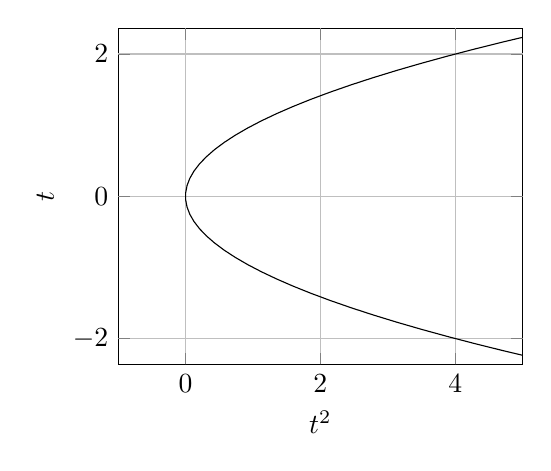
\begin{tikzpicture}
    \begin{axis}[view={0}{0}, xlabel=$ t^2 $, ylabel=$ t^3-3 $, zlabel=$t$, scale=0.75,
        xmin=-1,ymin=-2.5,xmax=5,ymax=2.5,grid]
        \addplot3[samples = 100, samples y = 0]
        ({x^2},{x^3-3*x},{x});
    \end{axis}
\end{tikzpicture}
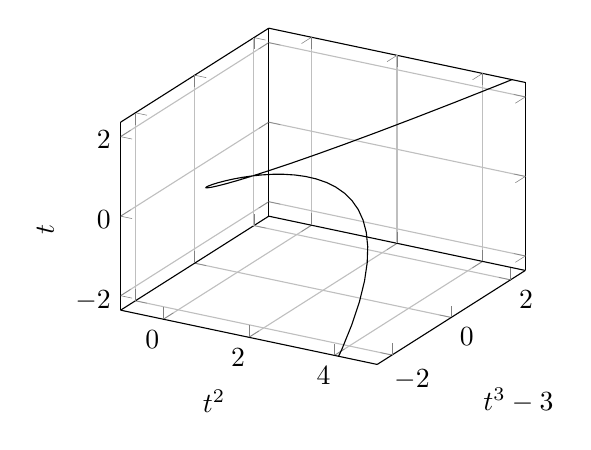
\begin{tikzpicture}
    \begin{axis}[view={30}{30}, xlabel=$ t^2 $, ylabel=$ t^3-3 $,zlabel=$t$, scale=0.75,
        xmin=-1,ymin=-2.5,xmax=5,ymax=2.5,grid]
        \addplot3[samples = 100, samples y = 0]
        ({x^2},{x^3-3*x},{x});
    \end{axis}
\end{tikzpicture}
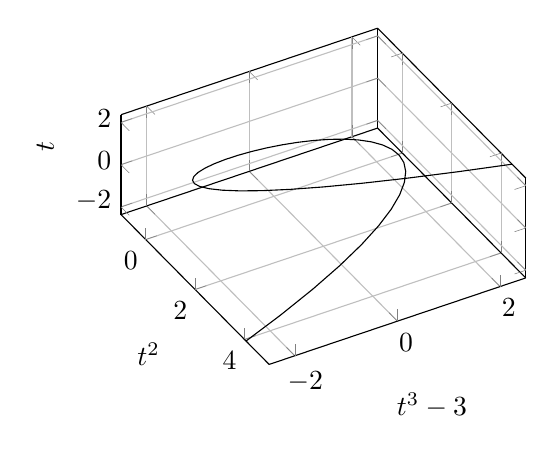
\begin{tikzpicture}
    \begin{axis}[view={60}{60}, xlabel=$ t^2 $, ylabel=$ t^3-3 $,zlabel=$t$, scale=0.75,
        xmin=-1,ymin=-2.5,xmax=5,ymax=2.5,grid]
        \addplot3[samples = 100, samples y = 0]
        ({x^2},{x^3-3*x},{x});
    \end{axis}
\end{tikzpicture}
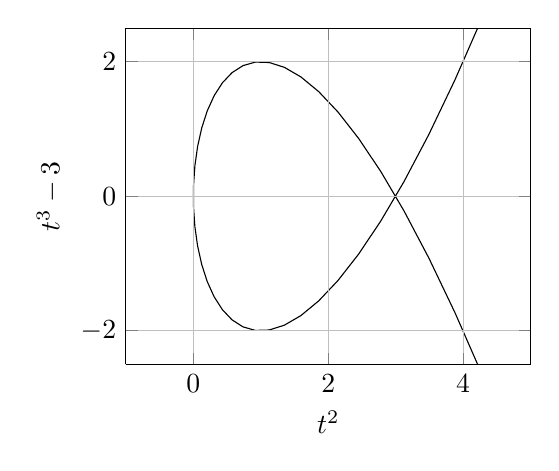
\begin{tikzpicture}
    \begin{axis}[view={0}{90}, xlabel=$ t^2 $, ylabel=$ t^3-3 $, scale=0.75,
        xmin=-1,ymin=-2.5,xmax=5,ymax=2.5,grid]
        \addplot3[samples = 100, samples y = 0]
        ({x^2},{x^3-3*x},{x});
    \end{axis}
\end{tikzpicture}
\newpage


\iffalse
\section{Spirals}
Using parametric curves you can create some really amazing spirals.

\begin{commentbox}{Archimedean spiral}
    $C = (t\cos(t), t\sin(t))$
\end{commentbox}
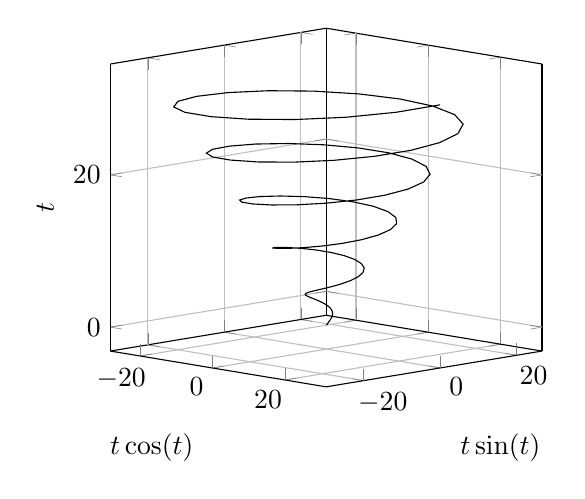
\begin{tikzpicture}
    \begin{axis}
        [
        scale=0.8,
        grid,
        view={45}{10},
        xlabel=$ t\cos(t) $,
        ylabel=$ t\sin(t) $,
        zlabel=$ t $,
        ]
    \addplot3[
        domain=0:10*pi,
        samples = 100,
        samples y=0,
    ]
    ({x*cos(deg(x))},
    {x*sin(deg(x))},
    {x});
    \end{axis}
\end{tikzpicture}


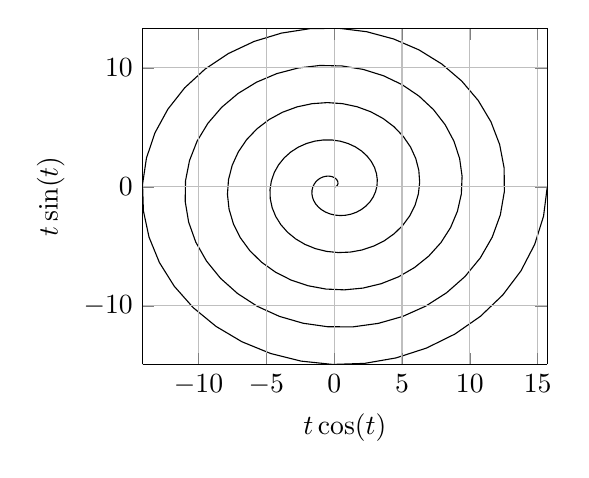
\begin{tikzpicture}
    \begin{axis}
        [scale=0.75,
        grid,
        view={0}{90},
        xlabel=$ t\cos(t) $,
        ylabel=$ t\sin(t) $,
        ]
    \addplot3[
        domain=0:10*pi,
        samples = 200,
        samples y=0,
    ]
    ({x*cos(deg(x))/2},
    {x*sin(deg(x))/2},
    {x});
    \end{axis}
\end{tikzpicture}

\begin{commentbox}{Hyperbolic spiral}
    $ C = \big(a \frac{\cos(t)}{t}, a \frac{\sin(t)}{t}\big),\ a = 5 $
\end{commentbox}

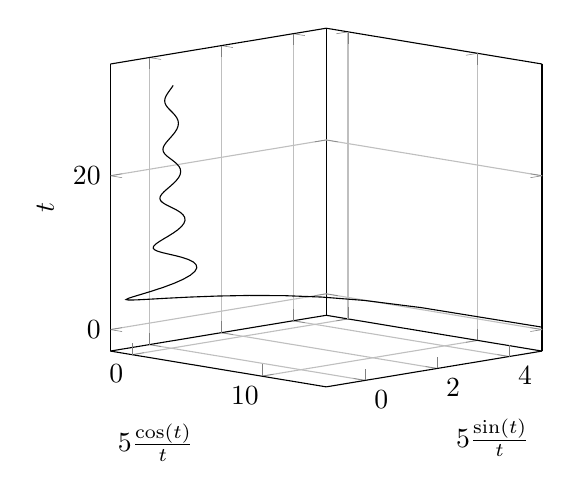
\begin{tikzpicture}
    \begin{axis}
        [
        scale=0.8,
        grid,
        view={45}{10},
        xlabel=$ 5\frac{\cos(t)}{t} $,
        ylabel=$ 5\frac{\sin(t)}{t} $,
        zlabel=$ t $,
        ]
    \addplot3[
        domain=0:10*pi,
        samples = 100,
        samples y=0,
    ]
    ({5*cos(deg(x))/x},
    {5*sin(deg(x))/x},
    {x});
    \end{axis}
\end{tikzpicture}
\newpage

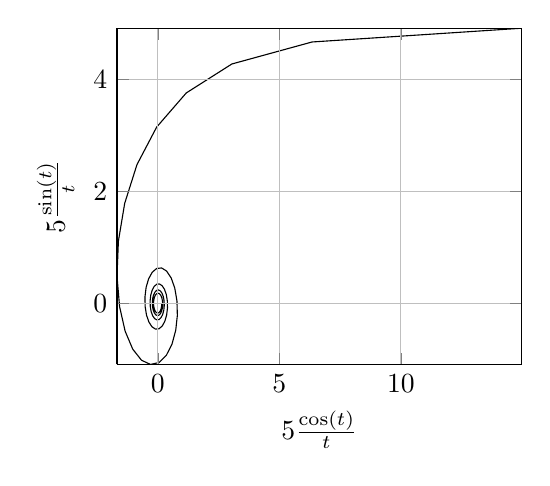
\begin{tikzpicture}
    \begin{axis}
        [scale=0.75,
        grid,
        view={0}{90},
        xlabel=$ 5\frac{\cos(t)}{t} $,
        ylabel=$ 5\frac{\sin(t)}{t} $,
        ]
    \addplot3[
        domain=0:10*pi,
        samples = 100,
        samples y=0,
    ]
    ({5*cos(deg(x))/x},
    {5*sin(deg(x))/x},
    {x});
    \end{axis}
\end{tikzpicture}

\begin{commentbox}{Fermat's spiral}
    $ C = (a \cdot \pm\sqrt{t}\cos(t), a \cdot \pm\sqrt{t}\sin(t)),\ a = 1 $
\end{commentbox}

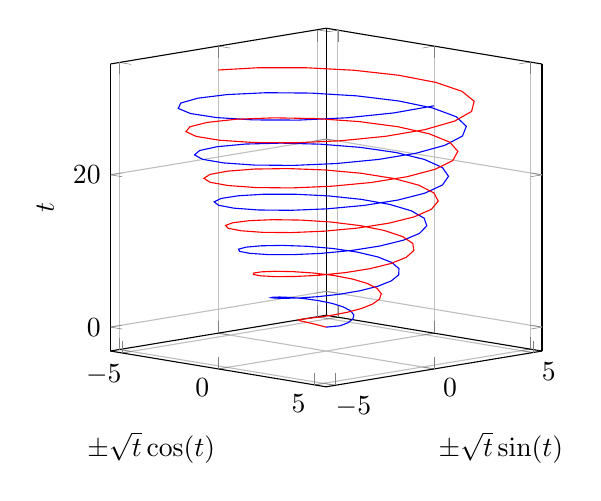
\begin{tikzpicture}
    \begin{axis}
        [
        scale=0.8,
        grid,
        view={45}{10},
        xlabel=$ \pm\sqrt{t}\cos(t) $,
        ylabel=$ \pm\sqrt{t}\sin(t) $,
        zlabel=$ t $,
        ]
    \addplot3[
        blue,
        domain=0:10*pi,
        samples = 100,
        samples y=0,
    ]
    ({sqrt(x)*cos(deg(x))},
    {sqrt(x)*sin(deg(x))},
    {x});
    \addplot3[
        red,
        domain=0:10*pi,
        samples = 100,
        samples y=0,
    ]
    ({-sqrt(x)*cos(deg(x))},
    {-sqrt(x)*sin(deg(x))},
    {x});
    \end{axis}
\end{tikzpicture}


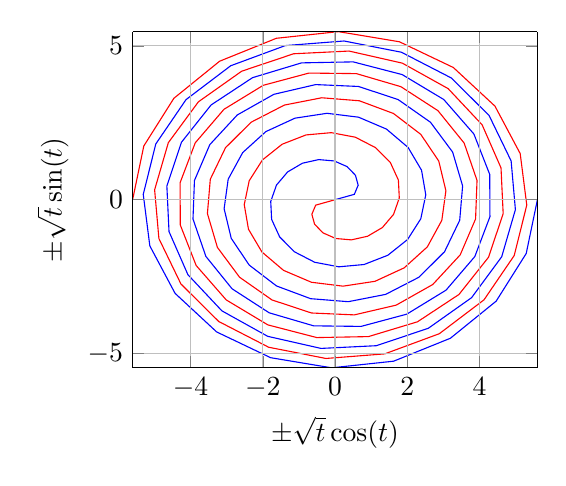
\begin{tikzpicture}
    \begin{axis}
        [scale=0.75,
        grid,
        view={0}{90},
        xlabel=$ \pm\sqrt{t}\cos(t) $,
        ylabel=$ \pm\sqrt{t}\sin(t) $,
        ]
    \addplot3[
        blue,
        domain=0:10*pi,
        samples = 100,
        samples y=0,
    ]
    ({sqrt(x)*cos(deg(x))},
    {sqrt(x)*sin(deg(x))},
    {x});
    \addplot3[
        red,
        domain=0:10*pi,
        samples = 100,
        samples y=0,
    ]
    ({-sqrt(x)*cos(deg(x))},
    {-sqrt(x)*sin(deg(x))},
    {x});
    \end{axis}
\end{tikzpicture}
\begin{commentbox}{Legend}
    \begin{itemize}
        \item The blue color is $ \sqrt{t}\cos(t),\ \sqrt{t}\sin(t) $
        \item The red color is $ -\sqrt{t}\cos(t),\ -\sqrt{t}\sin(t) $
    \end{itemize}
\end{commentbox}

\subsubsection{Summary}
You can make cool spirals using parametric curves.
\fi

\section{Area}
As we discussed before the the area underneath a function between two points is defined by the fundamental theorem of calculus i.e., $A = \int_a^b f(x)\ dx$.
\\~\\
We can use this same theorem to find the area of a parametric curve.
\\~\\
We know that 
$$
    \frac{dx}{dt} = x'(t)
$$
Therefore, $ dx = x'(t)\ dt $.
\\~\\
Substitute this into the fundamental theorem of calculus gives us this:
$$
    A = \int_a^b y\ x'(t)\ dt
$$
\begin{paperbox}{Area of a parametric curve}
    \begin{equation}
        A = \int_a^b y(t)x'(t)\ dt
    \end{equation}
    To find the area on the y-axis then use this equation:
    \begin{equation}
        A = \int_a^b x(t)y'(t)\ dt
    \end{equation}
\end{paperbox}
\subsubsection{Example}
Find the area of this parameter curve $ C = (t-\sin(t), 1-\cos(t)) $ from $ 0 \le t \le 2\pi $.
\paragraph{Solution}
\begin{gather*}
    x'(t) = 1-\cos(t)\ dt\\
    \int_0^{2\pi} (1-\cos(t))(1-\cos(t))\ dt\\
    \int_0^{2\pi} (1-\cos(t))^2\ dt\\
    \int_0^{2\pi} \cos^2(t) - 2\cos(t) + 1\ dt\\
    \int_0^{2\pi} \frac{1+\cos(2t)}{2} - 2\cos(t) + 1\ dt\\
    \frac{1}{2}t + \frac{1}{4}\sin(2t) - 2\sin(t) + t\biggl|_0^{2\pi}\\
    2\pi + \pi = 3\pi
\end{gather*}
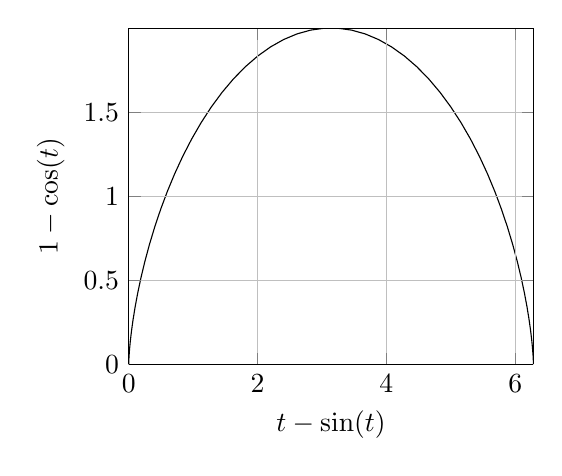
\begin{tikzpicture}
    \begin{axis}
        [scale=0.75,
        grid,
        view={0}{90},
        xlabel=$t-\sin(t)$,
        ylabel=$1-\cos(t)$,
        zlabel=$t$,
        ]
    \addplot3[
        domain=0:2*pi,
        samples = 60,
        samples y=0,
    ]
    ({x - sin(deg(x))},
    {(1 - cos(deg(x)))},
    {x});
    \end{axis}
\end{tikzpicture}

\section{Arc length}
Similar to $ L = \int_a^b \sqrt{1 + (f'(x))^2}\ dx $, but replace $dx$ with $ x'(t)\ dt $ and replace $ f'(x) $ with $ \frac{dy}{dx} $.
\begin{paperbox}{Arc length of a Parametric Curve}
    \begin{equation}
        L = \int_a^b \sqrt{(x'(t))^2+(y'(t))^2}\ dt
    \end{equation}
\end{paperbox}
\subsubsection{Example}
Find the arc length of this parametric curve $ C = (e^t-t, 4e^{t/2}) $ from 0 to 2. 
\paragraph{Solution}
\begin{gather*}
    x'(t) = e^t - 1,\ y'(t) = 2e^{t/2}\\
    \int_0^2 \sqrt{(e^t - 1)^2+(2e^{t/2})^2}\ dt\\
    \int_0^2 \sqrt{e^{2t} + 2e^t + 1}\ dt\\
    \int_0^2 \sqrt{(e^t + 1)^2}\ dt\\
    \int_0^2 e^t + 1\ dt\\
    e^t + t \biggl|_0^2\\
    e^2 + 1
\end{gather*}
\newpage

\section{Surface Area}
Similar to $ SA = \int_a^b 2\pi f(x) \sqrt{1 + (f'(x))^2}\ dx $, but replace $dx$ with $ x'(t)\ dt $ and replace $ f'(x) $ with $ \frac{dy}{dx} $.
\begin{paperbox}{Surface area of a Parametric Curve}
    \begin{equation}
        SA = \int_a^b 2\pi y(t) \sqrt{(x'(t))^2+(y'(t))^2}\ dt
    \end{equation}
\end{paperbox}
\subsubsection{Example}
Prove that the surface area of a sphere with radius $a$ is $ 4\pi a^2 $.
\paragraph{Solution}
The parametric curve for a semicircle with a radius $a$ is $ C = (a\cos(t), a\sin(t)) $ from $0 \le t \le \pi $.
\begin{gather*}
    x'(t) = -a\sin(t),\ y'(t) = a\cos(t)\\
    SA = \int_0^\pi 2\pi a\sin(t)\sqrt{(-a\sin(t))^2+(a\cos(t))^2}\ dt \\
    SA = \int_0^\pi 2\pi a\sin(t)\sqrt{a^2\sin^2(t)+a^2\cos^2(t)}\ dt \\
    SA = \int_0^\pi 2\pi a^2\sin(t)\sqrt{\sin^2(t)+\cos^2(t)}\ dt \\
    SA = \int_0^\pi 2\pi a^2\sin(t)\sqrt{1}\ dt \\
    SA = \int_0^\pi 2\pi a^2\sin(t)\ dt \\
    SA = 2\pi a^2 \int_0^\pi \sin(t)\ dt\\
    SA = 2\pi a^2 \biggl(-\cos(t)\biggl|_0^\pi\biggl)\\
    SA = 2\pi a^2 (-(-1) - (-1))\\
    SA = 2\pi a^2 (2)\\
    SA = 4\pi a^2
\end{gather*}
\hfill\ensuremath{\blacksquare}
\newpage

\section{Ellipse}
\begin{paperbox}{ellipse}
    Are parametric curves that encompasses all circles.
    \begin{equation}
        C = (a \cos(t), b \sin(t))\ \ a,b \in \mathbb{R}
    \end{equation}
    \begin{equation}
        \frac{x^2}{a^2} + \frac{y^2}{b^2} = 1
    \end{equation}
\end{paperbox}
\subsubsection{Example}
This is an ellipse where the parametric equation is $C = (\cos(t), 2\sin(t))$. As you can see the "radius" of the curve changes from 1 to 2.
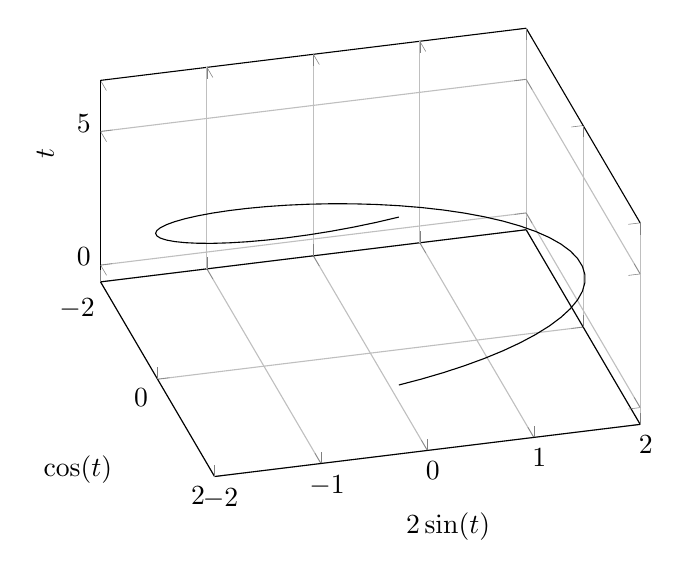
\begin{tikzpicture}
    \begin{axis}
        [
        grid,
        xmax=2,xmin=-2,
        view={75}{45},
        xlabel=$\cos(t)$,
        ylabel=$2 \sin(t)$,
        zlabel=$t$,
        ]
    \addplot3[
        domain=0:2*pi,
        samples = 60,
        samples y=0,
    ]
    ({cos(deg(x))},
    {(2*sin(deg(x)))},
    {x});
    \end{axis}
\end{tikzpicture}

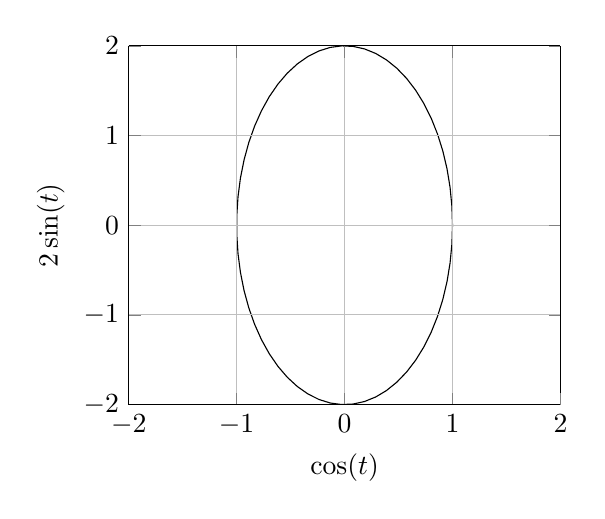
\begin{tikzpicture}
    \begin{axis}
        [
        scale=0.8,
        xmax=2,xmin=-2,
        grid,
        view={0}{90},
        xlabel=$\cos(t)$,
        ylabel=$2 \sin(t)$,
        zlabel=$t$,
        ]
    \addplot3[
        domain=0:2*pi,
        samples = 60,
        samples y=0,
    ]
    ({cos(deg(x))},
    {2*sin(deg(x))},
    {x});
    \end{axis}
\end{tikzpicture}

\newpage
\section{Hyperbolas}

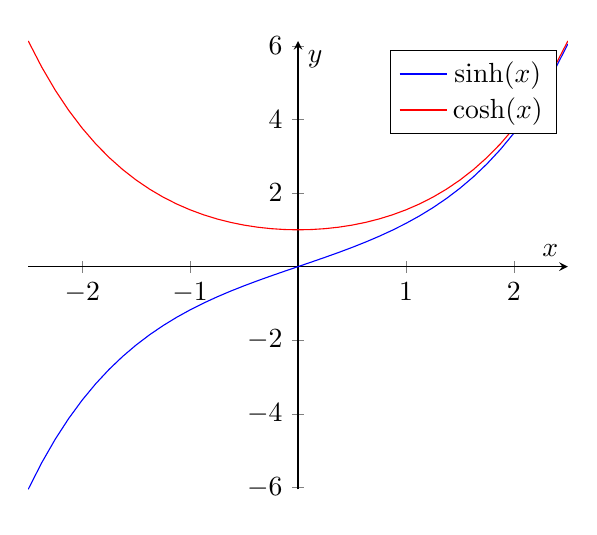
\begin{tikzpicture}
    \begin{axis}
        [
        axis lines = center,
        xlabel=$ x $,
        ylabel=$ y $,
        ]
        \addplot[blue, domain=-2.5:2.5, samples=41]
        {sinh(x)};
        \addlegendentry{$\sinh(x)$};
        \addplot[red, domain=-2.5:2.5, samples=41]
        {cosh(x)};
        \addlegendentry{$\cosh(x)$};
    \end{axis}
\end{tikzpicture}



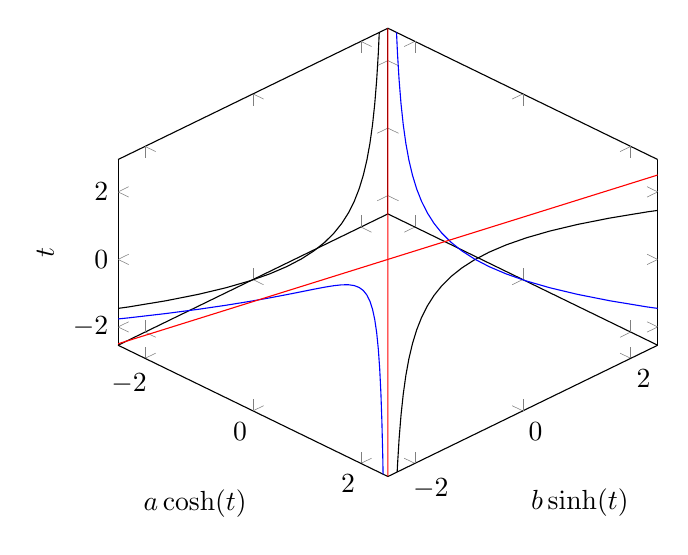
\begin{tikzpicture}
    \begin{axis}
        [
        xmin=-2.5, ymin=-2.5, xmax=2.5, ymax=2.5,
        view={45}{45},
        xlabel=$ a\cosh(t) $,
        ylabel=$ b\sinh(t) $,
        zlabel=$t$,
        ]
    \addplot3[
        domain=-pi:pi,
        samples = 41,
        samples y=0,
    ]
    ({cosh(x)},
    {sinh(x)},
    {x});
    \addplot3[
        domain=-pi:pi,
        samples = 41,
        samples y=0,
    ]
    ({-cosh(x)},
    {sinh(x)},
    {x});

    \addplot3[
        blue,
        domain=-pi:pi,
        samples = 41,
        samples y=0,
    ]
    ({sinh(x)},
    {-cosh(x)},
    {x});

    \addplot3[
        blue,
        domain=-pi:pi,
        samples = 41,
        samples y=0,
    ]
    ({-sinh(x)},
    {cosh(x)},
    {x});

    \addplot3[
        dotted, red,
    ]
    ({x},{x},{x});
    \addplot3[
        dotted, red,
    ]
    ({-x},{x},{x});
    \end{axis}
\end{tikzpicture}

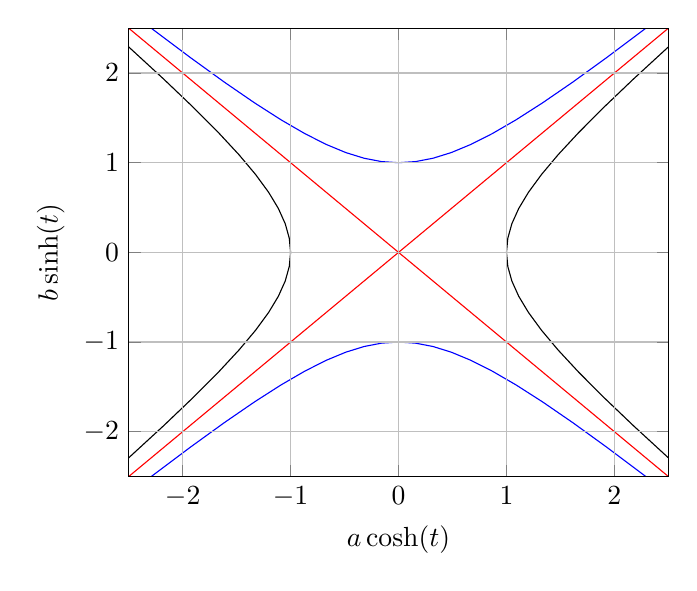
\begin{tikzpicture}
    \begin{axis}
        [
        xmin=-2.5, ymin=-2.5, xmax=2.5, ymax=2.5,
        grid, 
        view={0}{90},
        xlabel=$ a\cosh(t) $,
        ylabel=$ b\sinh(t) $,
        zlabel=$t$,
        ]
    \addplot3[
        domain=-pi:pi,
        samples = 41,
        samples y=0,
    ]
    ({cosh(x)},
    {sinh(x)},
    {x});
    \addplot3[
        domain=-pi:pi,
        samples = 41,
        samples y=0,
    ]
    ({-cosh(x)},
    {sinh(x)},
    {x});
    \addplot3[
        dashed, red,
    ]
    ({x},{x},{x});
    \addplot3[
        dashed, red,
    ]
    ({-x},{x},{x});
    \addplot3[
        blue,
        domain=-pi:pi,
        samples = 41,
        samples y=0,
    ]
    ({sinh(x)},
    {-cosh(x)},
    {x});

    \addplot3[
        blue,
        domain=-pi:pi,
        samples = 41,
        samples y=0,
    ]
    ({-sinh(x)},
    {cosh(x)},
    {x});
    \end{axis}

\end{tikzpicture}

\newpage

\section{Exercise}
\begin{enumerate}
    \item Consider the parametric equation below
    \[C = (x^2 - 2, t + 1),\ -3 \leq t \leq 3\]
    Find the arc length of the parametric equation using the domain provided.
    \item Consider the following parametric equation \[
        C = (\sin \left( \frac{1}{2} \theta\right), \cos\left( \frac{1}{2} \theta \right),\ -\pi \leq \tau \leq \pi)
    \] Find the arc length and the surface area of the parametric equation using the domain above
    \item Find an equation of the tangent to the curve at the point corresponding to the given value of the parameter \(x = t\cos(t),\ y = t\sin(t);\ t = \pi \)
    \item Find an equation of the tangent to the curve at the given point by both eliminating the parameter and without eliminating the parameter.\[
        x = 5 + \ln(t),\ y = t^2 + 8,\ (5,9)
    \]
    \item Find $ dy/dx $ and $ d^2y/dx^2 $ of this parametric equation 
    \[
        x = e^t,\ y = te^-t
    \] At which value of $t$ is the curve concave upward?
\end{enumerate}




\end{document}